\section{Evaluation of BoSSS for Viscid Flows}
\frame{\tableofcontents[currentsection]}
	\subsection{Theory}
	\begin{frame}
		\frametitle{Theory -- Differentiation into Flow Regimes}
		\begin{columns}[t]
			\column[]{5cm}
			\begin{itemize}
				\vspace{-1cm}
				\item $40-50 < \text{Re} < 190$: laminar vortex shedding,
				\item $190 < \text{Re} < 260$: \gls{3d} wake-transition regime,
			\end{itemize}
			\column[]{7cm}
			\begin{figure}[ht]
				%\centering
				 \vspace{-1cm}
				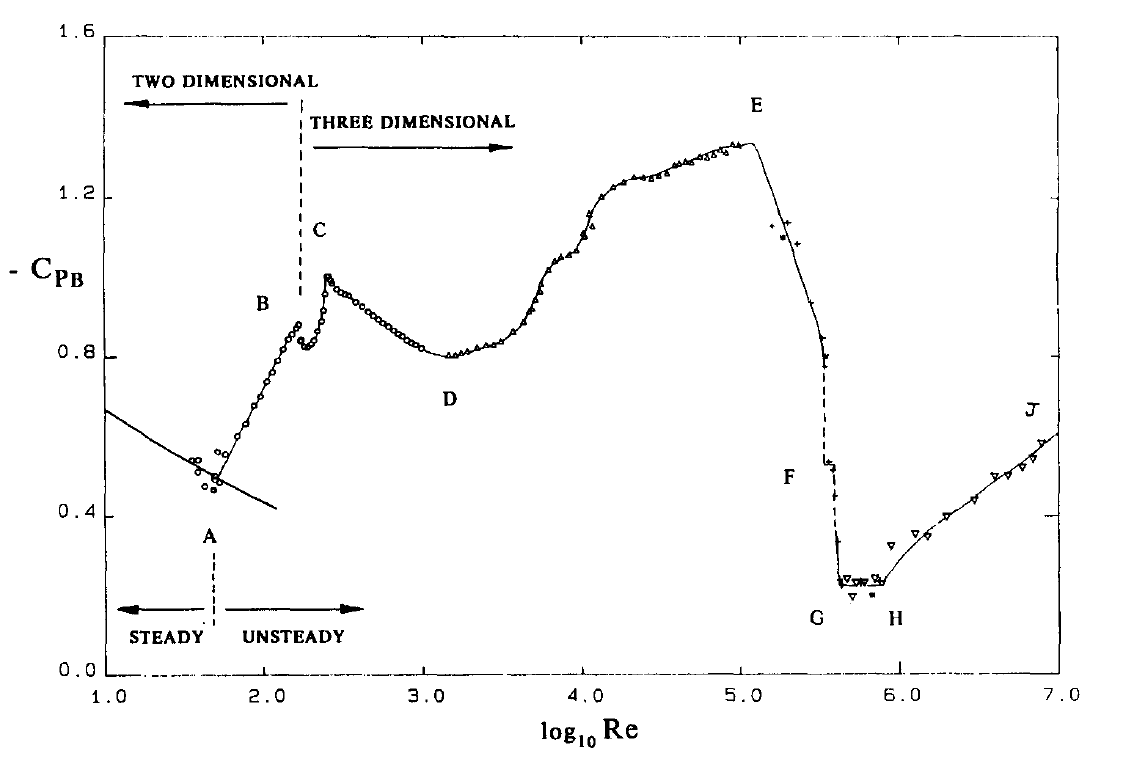
\includegraphics[width=\textwidth]{img/overviewCylinderReynolds_Williamson.PNG}
			\end{figure}
		\end{columns}
	\end{frame}
	\begin{frame}
		\frametitle{Theory -- Laminar Steady Regime}
		laminar steady regime
		Bild
		\begin{columns}[t]
		\column[]{7cm}
		\column[]{5cm}
		\begin{figure}[htbp]
			\vspace{-1cm}
			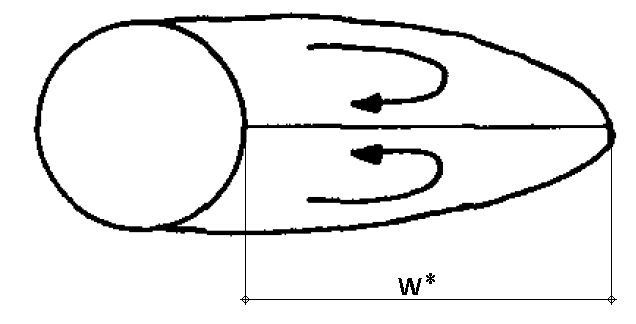
\includegraphics[width=\textwidth]{img/steadyFlow_modifiedWilliamson.PNG}
			\caption{Wake Separation Length, Taken from \cite{williamson1996vortex}, Modified }
			\label{fig:wakeSeparation}
		\end{figure} 
		\end{columns}

	\end{frame}	
	\begin{frame}
		\frametitle{Theory -- Laminar Vortex Shedding}
		Bild
		\begin{columns}[t]
			\column[]{5cm}
			\column[]{7cm}
			\begin{figure}[htbp]
				\vspace{-1cm}
				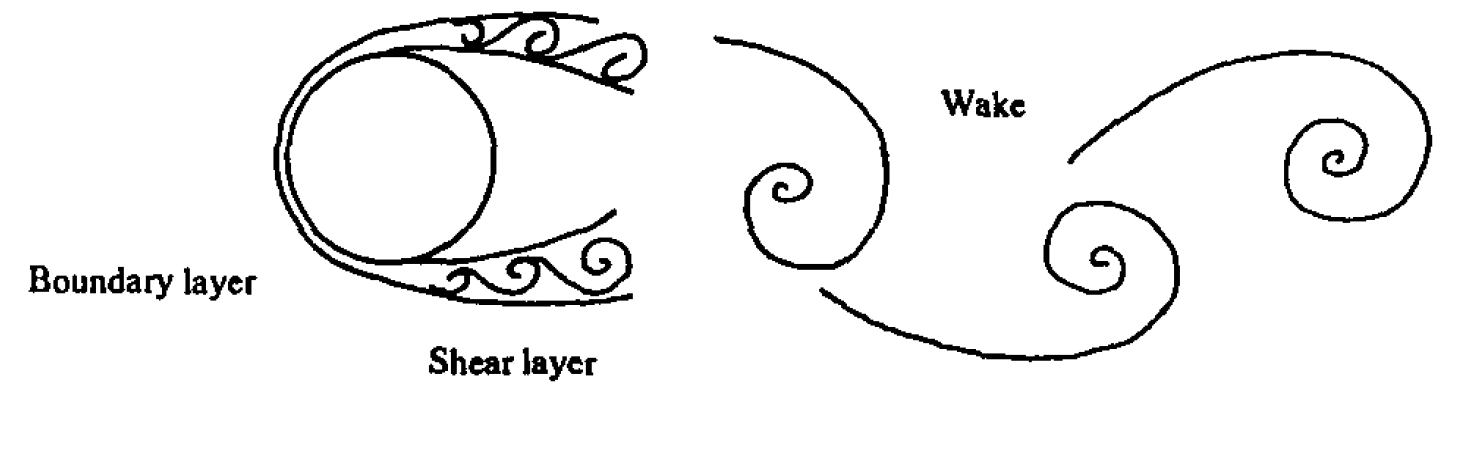
\includegraphics[width=\textwidth]{img/unsteady_Williamson.PNG}
				\caption{Kármán Vortex Street \cite{williamson1996vortex} }
				\label{fig:unsteady}
			\end{figure} 
		\end{columns}
		Karman vortex street
		frequency /strouhal
	\end{frame}	
	\subsection{Simulations}
		\begin{frame}
			\frametitle{Simulation Properties}
			simulation parameter
			gitter
			cD, CL, W*, St
		\end{frame}
		\begin{frame}[allowframebreaks]
			\frametitle{Simulation at $\text{Re = 20}$}
			\begin{table}[htp]
				\small
				\centering
				\begin{tabular}{|l|l|c|c|c|}
					\hline
					\rule{0pt}{2,3ex}$\text{Re}=20$                              & Source                             & \gls{2d}/\gls{3d} & $W^*$ & $C_D$ \\ \hline
					\rule{0pt}{2,3ex}\multirow{3}{*}{\begin{minipage}{2.8cm}Numerical --\newline Incompressible\end{minipage}} & \textcite{dennis1970numerical}           & \gls{2d}    & $0.94$     & $2.05$     \\ \cline{2-5} 
					\rule{0pt}{2,3ex}& \textcite{fornberg1980numerical}                 & \gls{2d}    & $0.91$     & $2.00$     \\ \cline{2-5} 
					\rule{0pt}{2,3ex}&\textcite{linnick2005high}          & \gls{2d}    &$ 0.93 $    & $2.06$     \\ \hline
					\rule{0pt}{2,3ex}\multirow{2}{*}{Experimental}               & \textcite{coutanceau1977experimental}       & -     & 0.93    & -     \\ \cline{2-5} 
					\rule{0pt}{2,3ex}& \textcite{tritton1959experiments}             & -     & -     & $2.09$     \\ \hline
					\rule{0pt}{2,3ex}\multirow{3}{*}{\begin{minipage}{2.8cm}Numerical --\newline Compressible\end{minipage}}     & \textcite{brehm2015locally} (Ma = 0.1) & \gls{3d}    & $0.96$     &$ 2.02$     \\ \cline{2-5} 
					\rule{0pt}{2,3ex}& \textcite{ayers}                 & \gls{2d}    & $0.975$     & $2.06 $    \\ \cline{2-5} 
					\rule{0pt}{2,3ex}& \textbf{Present Results:}                   & \gls{2d}    & $0.928$     & $2.136$     \\ \hline
				\end{tabular}	
				\caption{Comparison of Results for $W^*$ and $C_D$, taken from \cite{ayers}, modified}
				\label{tab:table20} 
			\end{table}
		%	re 20 tabelle, plot, drag over time, vorticity
		\end{frame}
		\begin{frame}
			\frametitle{Simulation at $\text{Re = 40}$}
			\begin{table}[htp]
				\small
				\centering
				\begin{tabular}{|l|l|c|c|c|}
					\hline
					\rule{0pt}{2,3ex}$\text{Re}=40$                              & Source                             & \gls{2d}/\gls{3d} & $W^*$ & $C_D$ \\ \hline
					\rule{0pt}{2,3ex}\multirow{3}{*}{\begin{minipage}{2.8cm}Numerical --\newline Incompressible\end{minipage}} &\textcite{dennis1970numerical}           & \gls{2d}    & $2.35$     & $1.52 $    \\ \cline{2-5} 
					\rule{0pt}{2,3ex}& \textcite{fornberg1980numerical}                & \gls{2d}    & $2.24$     & $1.50 $   \\ \cline{2-5} 
					\rule{0pt}{2,3ex}& \textcite{linnick2005high}          & \gls{2d}    &$ 2.28$     & $1.54  $   \\ \hline
					\rule{0pt}{2,3ex}\multirow{2}{*}{Experimental}               & \textcite{coutanceau1977experimental}      & -     & $2.13 $  & -     \\ \cline{2-5} 
					\rule{0pt}{2,3ex}& \textcite{tritton1959experiments}                 & -     & -     & $1.59 $    \\ \hline
					\rule{0pt}{2,3ex}\multirow{3}{*}{\begin{minipage}{2.8cm}Numerical --\newline Compressible\end{minipage}}     & \textcite{brehm2015locally} (Ma = 0.1) & \gls{3d}    & $2.26$     & $1.51 $    \\ \cline{2-5} 
					\rule{0pt}{2,3ex}& \textcite{ayers}                  & \gls{2d}    & $2.250 $    & $1.605$     \\ \cline{2-5} 
					\rule{0pt}{2,3ex}& \textbf{Present Results:}                   & \gls{2d}    & $2.201$     & $1.608 $    \\ \hline
				\end{tabular}	
				\caption{Comparison of Results for $W^*$ and $C_D$, taken from \cite{ayers}, modified}
				\label{table40}
			\end{table}
			re 40 tabelle, plot, drag over time, vorticity
		\end{frame}
		\begin{frame}
			\frametitle{Simulation at $\text{Re = 100}$}
			\begin{table}[H]
				\small
				\centering
				\begin{tabular}{|l|p{4cm}|c|c|c|c|}
					\hline
					\rule{0pt}{2,3ex}$\text{Re}=100$                              & Source                             & \gls{2d}/\gls{3d} & $St$ & $C_D$ & $C_L$\\ \hline
					\rule{0pt}{2,3ex}\multirow{7}{*}{\begin{minipage}{2.8cm}Numerical --\newline Incompressible\end{minipage}} & \textcite{gresho1984modified}           & \gls{2d}    & $0.18$     & $1.76$ & -   \\ \cline{2-6} 
					\rule{0pt}{2,3ex}&\textcite{linnick2005high} \newline ($\lambda = 0.056$)                 & \gls{2d}    & $0.169$     & $1.38 \pm 0.010$  &  $\pm  0.337 $\\ \cline{2-6} 
					\rule{0pt}{2,3ex}&\textcite{linnick2005high} \newline ($\lambda = 0.023$)                  & \gls{2d}    & $0.1696 $   & $1.34 \pm 0.009$  & $ \pm 0.333 $\\ \cline{2-6} 
					\rule{0pt}{2,3ex}&\textcite{FLM:14223}                  & \gls{2d}    & $0.165  $   &$ 1.253 $ & -  \\ \cline{2-6} 
					\rule{0pt}{2,3ex}& \textcite{saiki1996numerical}                 & \gls{2d}    &$ 0.171  $   & $1.26 $ &  - \\ \cline{2-6} 
					\rule{0pt}{2,3ex}& \textcite{FLM:14223}                    & \gls{3d}    & $0.164$     & $1.240 $ & -  \\ \cline{2-6} 
					\rule{0pt}{2,3ex}& \textcite{liu1998preconditioned}          & \gls{3d}    &$ 0.165 $    & $1.35 \pm 0.012$  &$ \pm 0.339 $ \\ \hline
					\rule{0pt}{2,3ex}\multirow{2}{*}{Experimental}               & \textcite{berger1972periodic}     & -     &$ 0.16-0.17 $   & -    & -\\ \cline{2-6} 
					\rule{0pt}{2,3ex}& \textcite{clift2005bubbles}                & -    & -     &$ 1.24 $ &  - \\ \cline{2-6} 
					\rule{0pt}{2,3ex}& \textcite{williamson1996vortex}               & -     &$ 0.164  $  & -   & - \\ \hline
					\rule{0pt}{2,3ex}\multirow{3}{*}{\begin{minipage}{2.8cm}Numerical -- \newline Compressible\end{minipage}}     & \textcite{brehm2015locally} \newline (Ma = 0.1) & \gls{3d}    & $0.165$    &$ 1.32 \pm 0.01  $  & $\pm 0.32 $\\ \cline{2-6} 
					\rule{0pt}{2,3ex}& \textcite{ayers}                  & \gls{2d}    &$ 0.167$     & $1.371 \pm 0.011 $ &$ \pm 0.333 $\\ \cline{2-6} 
					\rule{0pt}{2,3ex}& \textbf{Present Results:}                   & \gls{2d}    & $0.1669$     & $1.3593 \pm 0.00805$  &  $\pm 0.3291$ \\ \hline
				\end{tabular}	
				\caption{Comparison of Results for $St$, $C_D$ and $C_L$, taken from \cite{ayers}, modified}
				\label{table100}
			\end{table}
			re 100 tabelle, plot, lift over time, vorticity
		\end{frame}
		\begin{frame}
			\frametitle{Simulation at $\text{Re = 200}$}
			\begin{table}[htp]
				\small
				\centering
				\begin{tabular}{|l|c|c|c|c|c|}
					\hline
					\rule{0pt}{2,3ex}$\text{Re}=200$                              & Source                             & \gls{2d}/\gls{3d} & $St$ & $C_D$ & $C_L$\\ \hline
					\rule{0pt}{2,3ex}\multirow{9}{*}{\begin{minipage}{2.8cm}Numerical --\newline Incompressible\end{minipage}} & \textcite{belov1995new}            & \gls{2d}    & $0.193$     & $1.19 \pm 0.042$ & $\pm 0.64$   \\ \cline{2-6} 
					\rule{0pt}{2,3ex} & \textcite{gresho1984modified}             & \gls{2d}    & $0.21$     & $1.76$ & -   \\ \cline{2-6} 
					\rule{0pt}{2,3ex}&\textcite{linnick2005high} \newline ($\lambda = 0.056$)                 & \gls{2d}    & $0.199$     & $1.37 \pm 0.046$  &  $\pm  0.70$\\ \cline{2-6} 
					\rule{0pt}{2,3ex}&\textcite{linnick2005high} \newline ($\lambda = 0.023$)                  & \gls{2d}    & $0.197 $   & $1.34 \pm 0.044$  & $ \pm 0.69$\\ \cline{2-6} 
					\rule{0pt}{2,3ex}& \textcite{miyake1992numerical}               & \gls{2d}    & $0.196$   &$1.34 \pm 0.043 $ & $\pm 0.67$  \\ \cline{2-6} 
					\rule{0pt}{2,3ex}&  \textcite{FLM:14223}               & \gls{2d}    & $0.198  $   &$ 1.321 $ & -  \\ \cline{2-6} 
					\rule{0pt}{2,3ex}&\textcite{saiki1996numerical}                 & \gls{2d}    &$ 0.197  $   & $1.18 $ &  - \\ \cline{2-6} 
					\rule{0pt}{2,3ex}& \textcite{FLM:14223}                   & \gls{3d}    & $0.181$     & $1.306 $ & -  \\ \cline{2-6} 
					\rule{0pt}{2,3ex}&\textcite{liu1998preconditioned}           & \gls{3d}    &$ 0.192 $    & $1.31 \pm 0.049$  &$ \pm 0.69 $ \\ \hline
					\rule{0pt}{2,3ex}\multirow{2}{*}{Experimental}               & \textcite{berger1972periodic}      & -     &$ 0.18-0.19 $   & -    & -\\ \cline{2-6} 
					\rule{0pt}{2,3ex}& \textcite{clift2005bubbles}                  & -    & -     &$ 1.16 $ &  - \\ \cline{2-6} 
					\rule{0pt}{2,3ex}& \textcite{williamson1996vortex}               & -     &$ 0.181  $  & -   & - \\ \hline
					\rule{0pt}{2,3ex}\multirow{3}{*}{\begin{minipage}{2.8cm}Numerical --\newline Compressible\end{minipage} }    &  \textcite{brehm2015locally} \newline (Ma = 0.1) & \gls{3d}    & $0.192$    &$ 1.3 \pm 0.04  $  & $\pm 0.66 $\\ \cline{2-6} 
					\rule{0pt}{2,3ex}& \textcite{ayers}                   & \gls{2d}    &$ 0.201$     & $1.371 \pm 0.011 $ &$ \pm 0.70 $\\ \cline{2-6} 
					\rule{0pt}{2,3ex}& \textbf{Present Results:}                   & \gls{2d}    & $0.2002$     & $1.344 \pm 0.0462$  &   $\pm 0.6887$\\ \hline
				\end{tabular}	
				\caption{Comparison of Results for $St$, $C_D$ and $C_L$, taken from \cite{ayers}, modified}
				\label{table200}
			\end{table}
			re 200 tabelle, plot, lift over time, vorticity
		\end{frame}